%%%%%%%%%%%%%%%%%%%%%%%%%%%%%%%%%%%%%%%%%%%%%%%%%%%%%%%%%%%%%%%%%%% 
%                                                                 %
%                            CHAPTER                              %
%                                                                 %
%%%%%%%%%%%%%%%%%%%%%%%%%%%%%%%%%%%%%%%%%%%%%%%%%%%%%%%%%%%%%%%%%%% 
\chapter{Implementation}
\label{chapter:implementation}
In this chapter we present the design, limitations and implementation of the proposed system. The design and any of its components are not bound to any specific technology, as such they can be implemented using any programming language, framework or mapping language. Using a mapping outside its intended purpose has some limitations, we present these fundamental limitations in their own section. For the implementation we first present the general setup of the environment. We then present the implementation of the data retrieval. Lastly we present some implementations of template creation and filling.

\section{System Design}
The system we propose is a pipeline that takes as input a knowledge graph and set of mapping rules and outputs the source files from which it would have been constructed. It has the advantage of being very modular, consisting of separate data retrieval and template creation/filling modules. The data retrieval module takes a mapping file and a knowledge graph, and outputs a table with the necessary data. The templating module will take the same mapping file and the table outputted by the data retrieval module and output a source file. Depending on the mapping rules and config files different modules will be used. The graph source will decide the data retrieval strategy while the output file will determine the templating engine to be used. An overview of the design can be seen in figure \ref{fig:design}.

We will implement the system in Python, using the Morph-KGC library to process the mapping rules. For the data retrieval module, we use RML to generate SPARQL queries to execute on a SPARQL endpoint (which we set up if necessary). This gives us a single table of data in CSV format for each source which we load into a Pandas DataFrame, which is then passed on to one of two templating modules we implement: one for tabular data (CSV) and one for nested/tree data (JSON). The structure for the templates is reconstructed from the RML mapping rules. Our specific implementation is shown in figure \ref{fig:specific_design}.

\begin{figure}
    \centering
    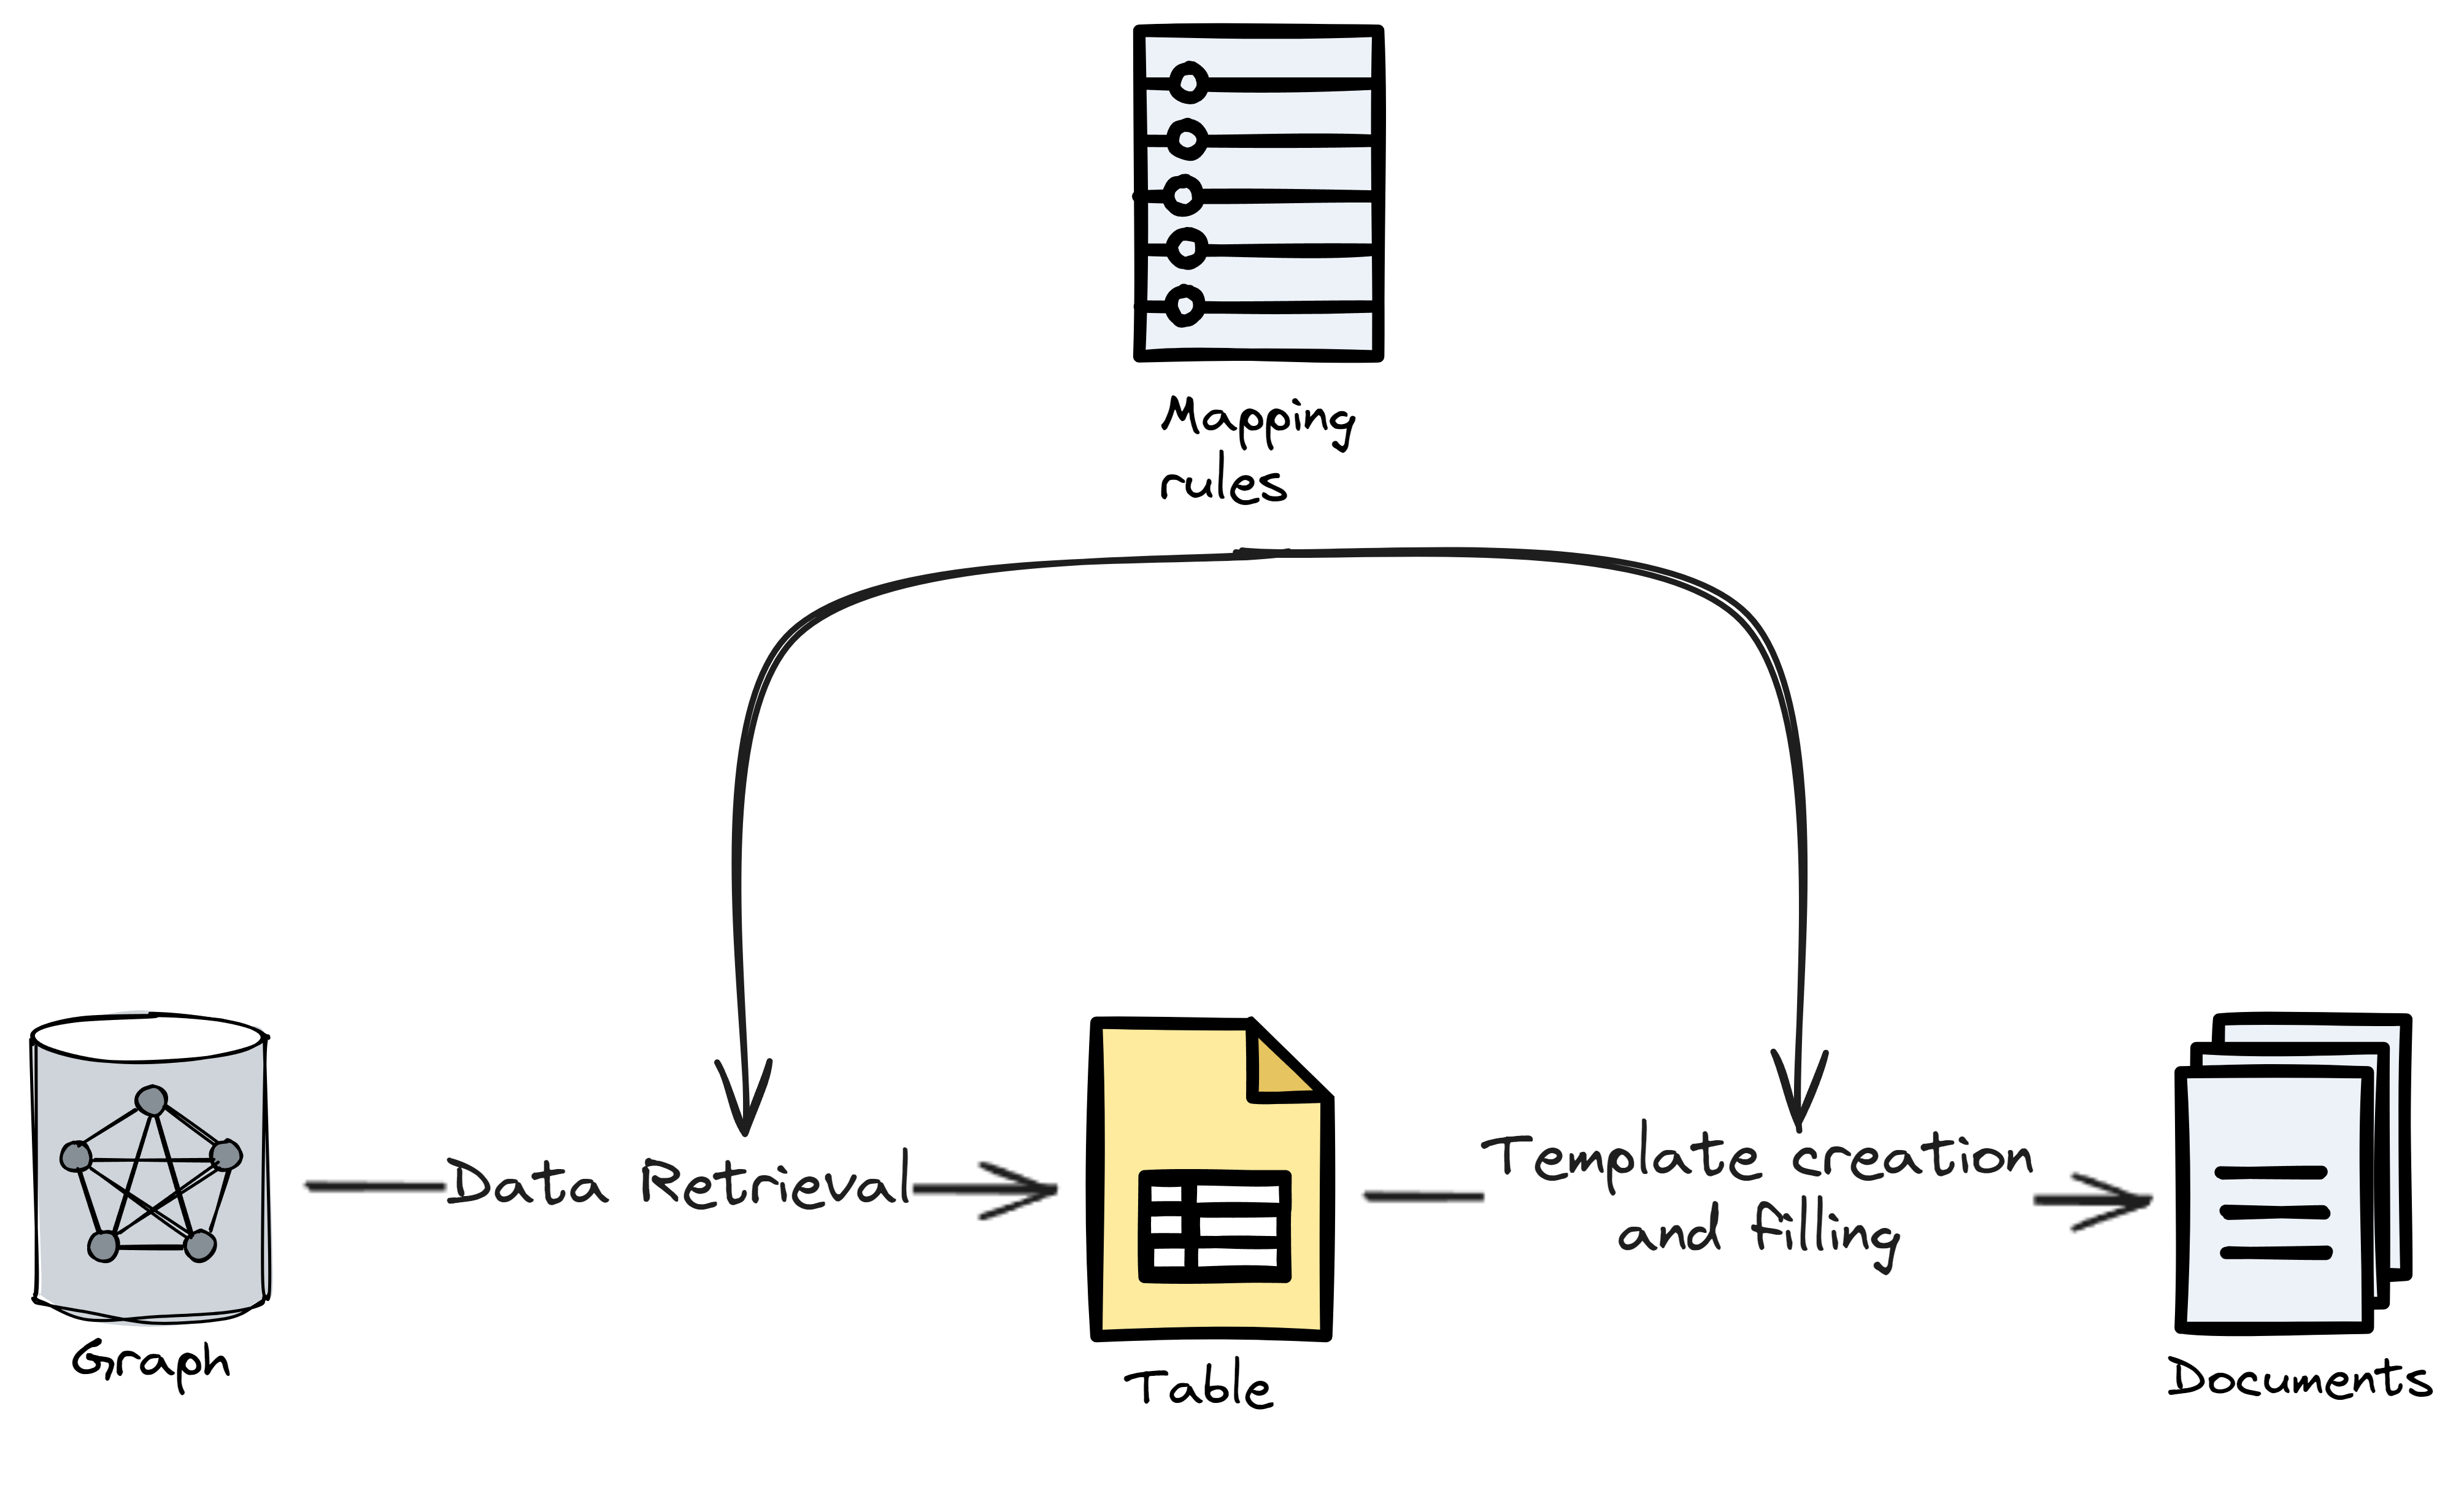
\includegraphics[width=0.9\textwidth]{fig/design.png}
    \caption{Design of the proposed system}
    \label{fig:design}   
\end{figure}

\begin{figure}
    \centering
    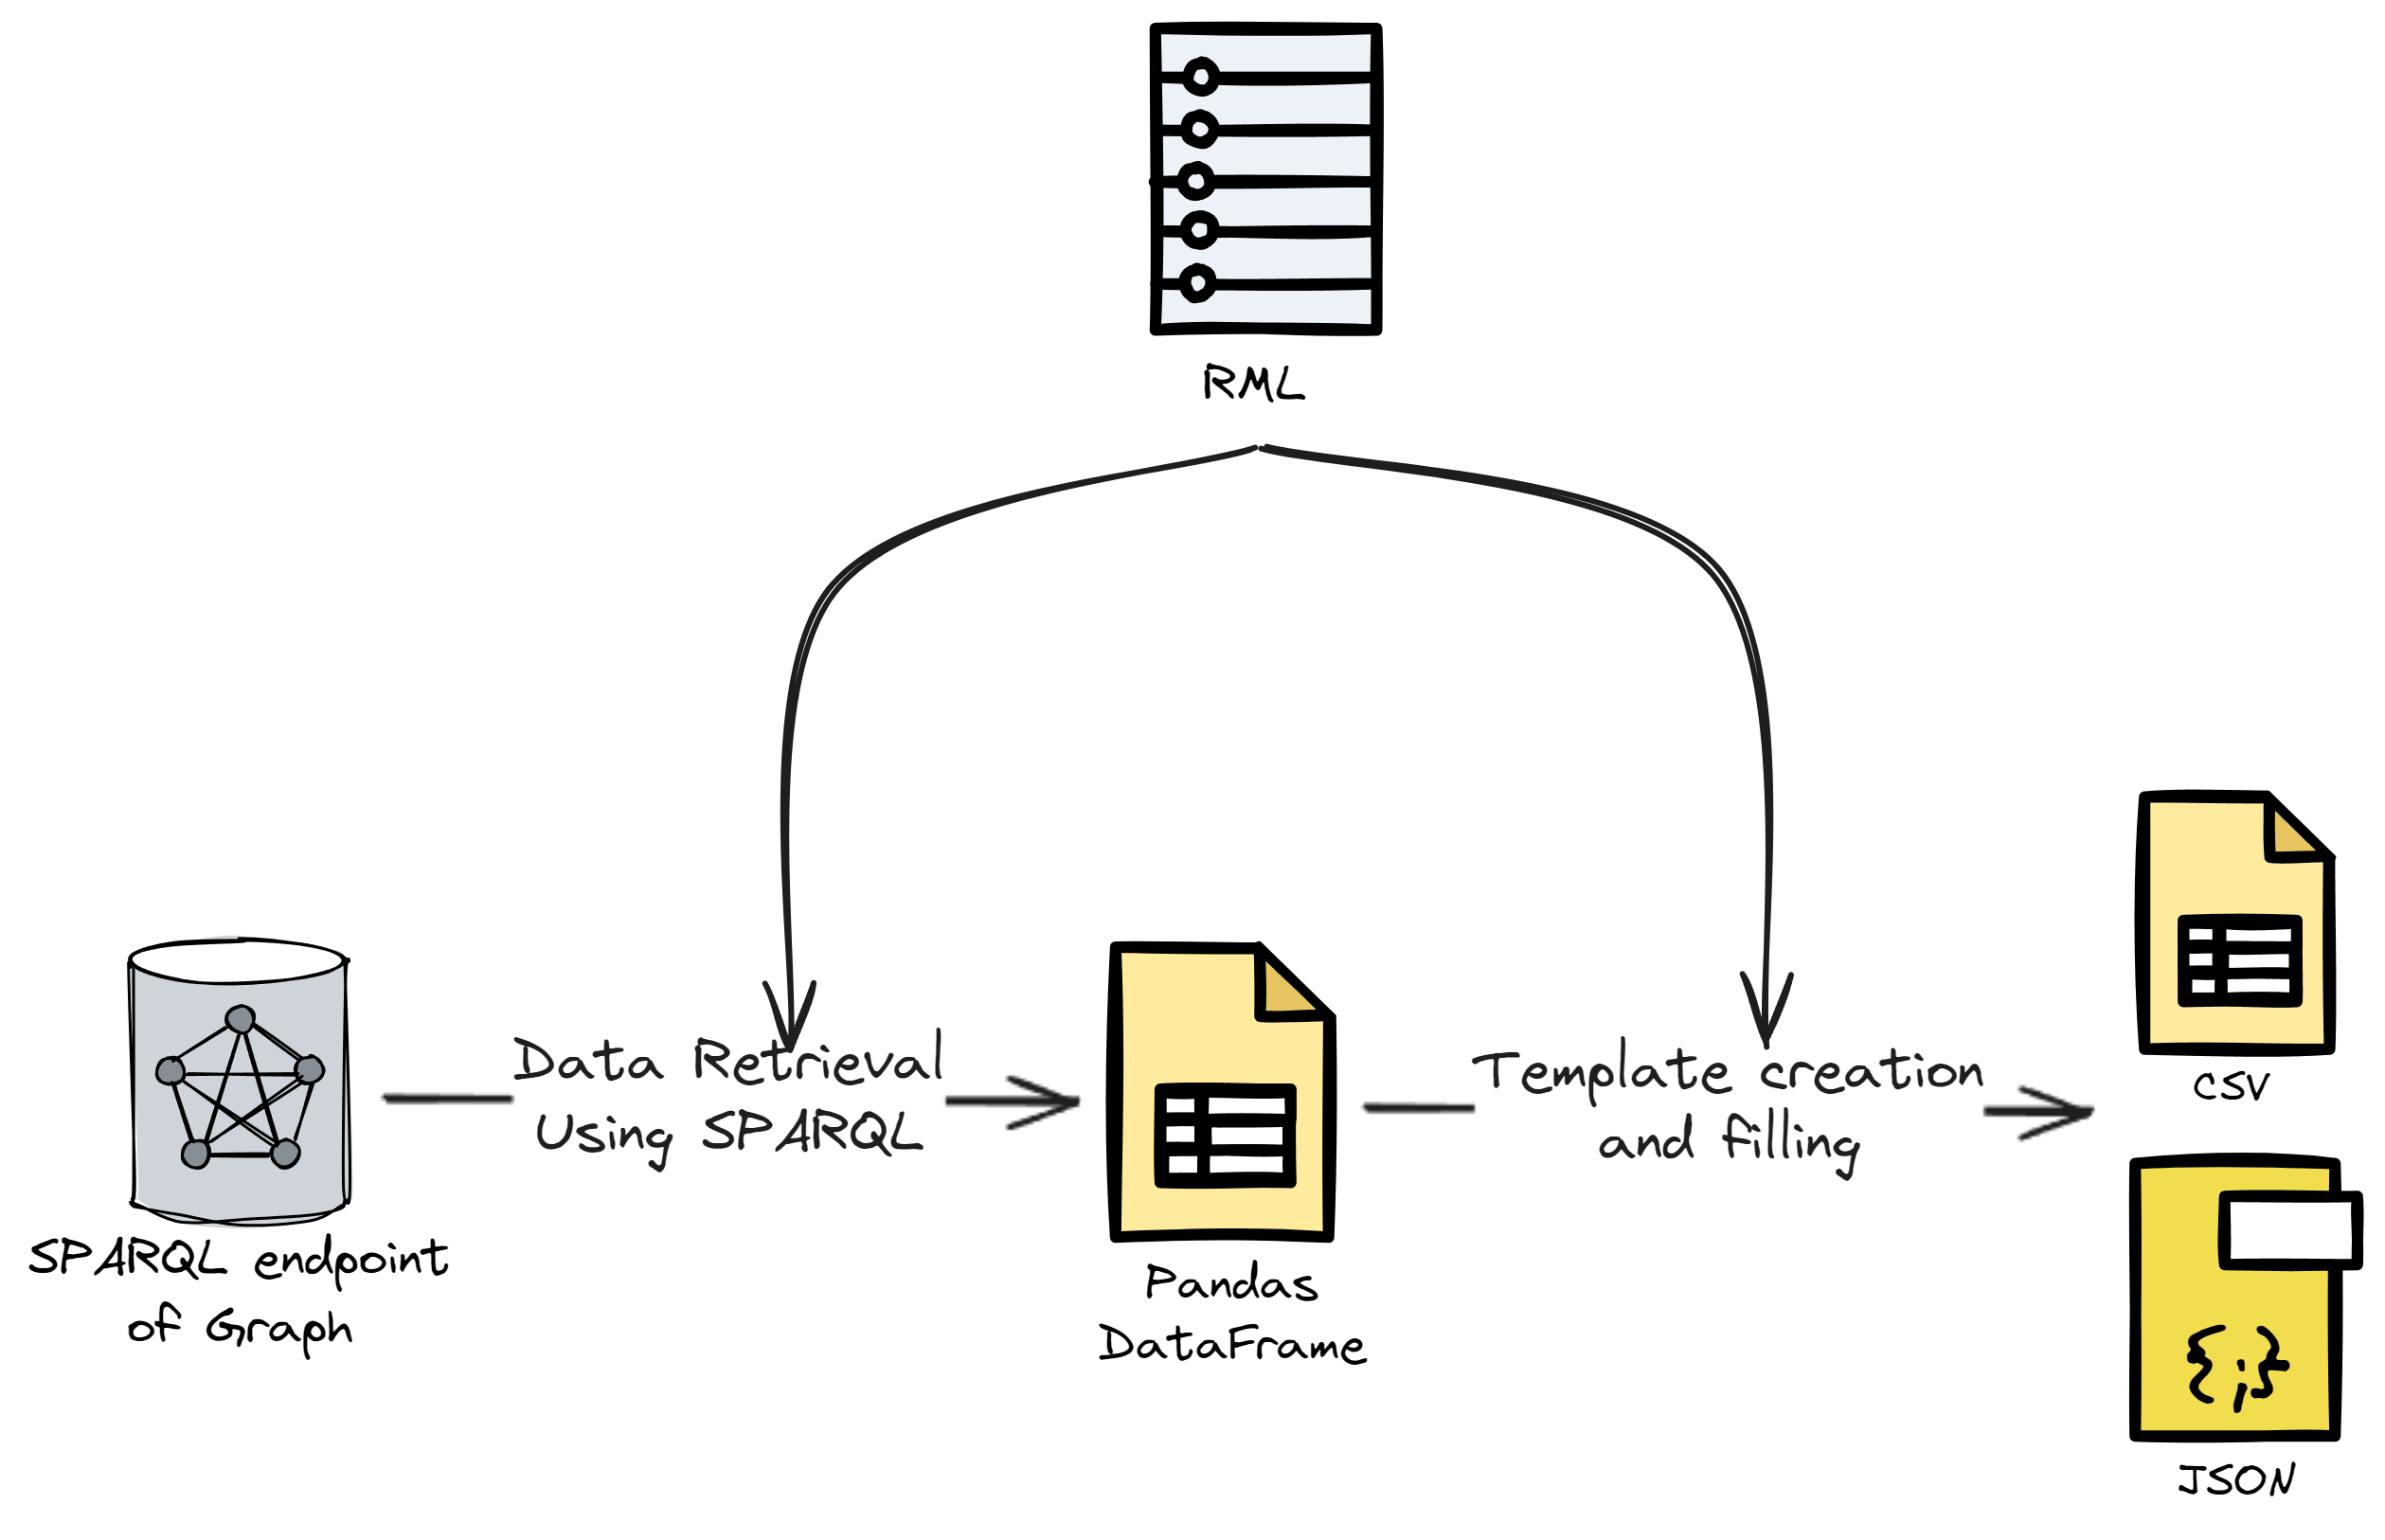
\includegraphics[width=0.9\textwidth]{fig/specific_design.png}
    \caption{Specific implementation of the design}
    \label{fig:specific_design}
\end{figure}

\section{System limitations}
\label{section:limitations}

We observe three types of limitation inherent to the system. As they stem from the very basis of the system, some are impossible to overcome while others can be mitigated. The first two are caused by irreversible processing, transforming the source or data in such a way that it is impossible to reconstruct the original. The third is caused by the design of nested data structures, where the method of data access can limit the ability to reconstruct the source.

\subsection{Irreversible source transformation}
\label{subsection:irreversible_source_transformation}
The first limitation is caused by the transformation of the source data before mapping. The most common irreversible transformation of a source in RML is a view over a database. While some views could be reversible, like a simple projection, many are not. To be able to fully recreate a static source it must be passed on in full to the mapper, without any aggregation, filtering, or other irreversible transformations. To update an existing source, having a unique identifying (set of) reference would suffice, for databases this would be the primary key(s). The mapping must also use all the data in the table. An example irreversible source mapping on a database can be found in listing \ref{lst:irreversible_source_mapping}. This limitation is not limited to database sources. Query languages working on data formats like JSON or XML also have the capability to filter or select data, making full reconstruction impossible. Some examples of this can be found in table \ref{table:irreversible_source_mapping}.

\begin{lstlisting}[caption={Irreversible source mapping from R2RML Test cases}, label={lst:irreversible_source_mapping}, captionpos=b, basicstyle=\small, frame=single]
<TriplesMap1>
    a rr:TriplesMap;
        
    rr:logicalTable [ rr:sqlQuery """
        SELECT "Name", COUNT("Sport") as SPORTCOUNT
        FROM "Student"
        """ ];

    rr:subjectMap [ rr:template 
                    "http://example.com/resource/student_{\"Name\"}"; ]; 

    rr:predicateObjectMap
    [ 
        rr:predicate	foaf:name ; 
        rr:objectMap	[ rr:column "\"Name\""; ];
    ];

    rr:predicateObjectMap
    [ 
		rr:predicate	ex:numSport ; 
		rr:objectMap	[ rr:column "SPORTCOUNT"; ];
    ];
    .
\end{lstlisting}

\begin{table}[!ht]
    \begin{tabular}{|lll|}
    \hline
    XPath            & JSONPath               & Description                       \\ \hline
    //book[last()]       & \begin{tabular}[c]{@{}l@{}}\$..book[(@.length-1)]\\  \$..book[-1:]\end{tabular} & the last book in order. \\ \hline
    //book[position()$<$3] & \begin{tabular}[c]{@{}l@{}}\$..book[0,1]\\  \$..book[:2]\end{tabular}           & the first two books     \\ \hline
    //book[isbn]     & \$..book[?(@.isbn)]     & filter all books with isbn number \\ \hline
    //book[price$<$10] & \$..book[?(@.price$<$10)] & filter all books cheaper than 10 \\ \hline
    \end{tabular}
    \caption{Examples of irreversible source access in XPath and JSONPath}
    \label{table:irreversible_source_mapping}
\end{table}

\subsection{Irreversible data transformation}
\label{subsection:irreversible_data_transformation}
The second limitation is caused by the transformation of data during mapping. RML allows for the transformation of data using functions. These functions offer a lot of functionality, from string functions (concat, replace, etc.) to math to custom (self-defined) functions. The result of these functions can either be stored in the graph as a value or used to join data. This transformation is often irreversible, with information from the original data lost. Take for example \texttt{grel:toUpperCase}: this function transforms the string to an all uppercase string, here we lose information about the original case. 

A special instance of this is the use of template maps. Template maps are a feature of most mapping languages, either explicitly (\texttt{d2rq:pattern}, \texttt{rr:template}) or implicitly through custom functions. These maps allow for the composition of multiple references into a single value using a template. This can be used to create both \acrshortpl{uri} (e.g. \texttt{http://example.com/resource/student\_\{"Name"\}\_\{"First Name"\}}) or literal values (e.g. \texttt{"\{"Name"\} \{"First Name"\}"}). For literal values this operation is theoretically irreversible as no guarantees can be made about the contents of the original data. Only by being sure the separator between the references consist of a pattern not present in the theoretical reconstructed source can we reliably split the value back into its original references. So to find out if we can reliably reconstruct the source we need the source, creating a chicken and egg problem. For \acrshortpl{uri} the operation is reversible if the separator consists of ``reserved characters" defined by rfc3986 \citep{rfc3986}, these are as follows: \texttt{:/?\#[]@!\$\&'()*+,;=}.

\subsection{Unreconstructable data structures}
The third limitation is caused by the design of nested data structures. To access the data multiple paths are valid to retrieve the data. The examples in table \ref{table:irreversible_source_mapping} also apply here, as they use 'recursive descent' to access the data. In the example any element with the name 'book' is taken from the JSON, no matter the depth. Alternatively a direct path could be written out like \texttt{\$.store.book.title}. Another valid option for this particular dataset would be to use wildcard operators like \texttt{\$.*.*.title}. Only a direct path gives us enough information to reconstruct the source file using the mapping rules. A recursive descent gives no indications as to the depth of the results, and using wildcards gives no information about the naming of the elements. While a 'suggested' source file could still be reconstructed, and it would still work with the mapping rules, it would almost certainly not share the same structure as the original source.

\section{Setup}

We choose to make our implementation in Python as it both has an extensive set of libraries and is well suited for rapid development. We use Morph-KGC to process the mapping rules for its ease of use, being well made and its use of the pandas library to represent the mapping rules. As the graph source we choose a standalone SPARQL endpoint on a triple store. For working with graph (\acrshort{rdf}) files, we first upload them to a triple store.

First the endpoint is set up, if necessary. If the source is a file, it is uploaded to the endpoint using the SPARQL 1.1 Graph Store HTTP Protocol. In our setup this is a locally running free version of GraphDB. The url of the repository is then wrapped using the SPARQLWrapper library and some settings are set.

Next we load the mapping rules from the mapping(\acrshort{rml}) files using Morph-KGC's internal \texttt{retrieve\_mappings} function. This function takes a config file (.ini format) as input, which specifies the location of the mapping files and various other settings which can be used to configure the behavior of the mapping. The mappings are returned as a pandas DataFrame which we enrich with various helper columns. An example of a single mapping rule (row in the DataFrame) can be found in listing \ref{lst:mapping_rule}. Marked in bold are the helper columns we add.

\begin{lstlisting}[caption={Example of a mapping rule in Morph-KGC}, label={lst:mapping_rule}, captionpos=b, basicstyle=\small, frame=single]
source_name: DataSource1
triples_map_id: #TM0
triples_map_type: http://w3id.org/rml/TriplesMap
logical_source_type: http://w3id.org/rml/source
logical_source_value: student.csv
iterator: nan
subject_map_type: http://w3id.org/rml/template
subject_map_value: http://example.com/{Name}
[*subject_references_template: http://example.com/([^\/]*)$*]
[*subject_references: ['Name']*]
[*subject_reference_count: 1*]
subject_termtype: http://w3id.org/rml/IRI
predicate_map_type: http://w3id.org/rml/constant
predicate_map_value: http://xmlns.com/foaf/0.1/name
[*predicate_references_template: None
predicate_references: []
predicate_reference_count: 0*]
object_map_type: http://w3id.org/rml/reference
object_map_value: Name
[*object_references_template: None
object_references: ['Name']
object_reference_count: 1*]
object_termtype: http://w3id.org/rml/Literal
object_datatype: nan
object_language: nan
graph_map_type: http://w3id.org/rml/constant
graph_map_value: http://w3id.org/rml/defaultGraph
subject_join_conditions: nan
object_join_conditions: nan
source_type: CSV
mapping_partition: 1-1-1-1
\end{lstlisting}

\section{Retrieving the data}
\label{section:retrieving_data}
Retrieving the data is done by querying the \acrshort{sparql} endpoint using an automatically generated query. All the required data from the source is retrieved at once. This does result in some degree of duplication for nested structures, but doing all processing and joining server-side is preferable. This sadly has a disadvantage of disjointed mappings currently resulting in a Cartesian product of the fragments. This is further discussed in subsection \ref{subsection:disjointed_mappings}. The data is returned as a CSV-table which is then loaded into a pandas DataFrame for further processing. The only post processing done is the decoding of url-encoded strings where necessary. 

\subsection{Generating the queries}
\label{subsection:generating_queries}
To generate the queries we first select the triple maps we want to use to generate the query. While constant values are always included, we can lighten the load on the server and in some cases increase reliability by reducing the amount and complexity of mapping rules we use. We design three operating modes:
\begin{itemize}
    \item \textbf{Full}: All triple maps are used to generate the query. This is the most complete mode, where all present instance of each reference is checked. Template maps can cause issues when the template is properly not reversible.
    \item \textbf{Reduced}: All triple maps with a object map type of reference are used to generate the query. Only where necessary to retrieve all data template map types are used to try and avoid the issues with their reversibility.
    \item \textbf{Minimal}: Only a single datapoint is used for each reference, with a preference for reference object map types. This further reduces the load on the server and the complexity of the query. 
\end{itemize}

We then generate the queries by translating the mapping rules into patterns. 
Each of the three map types, constant, reference, and template, generates a different pattern.
For the constant map type, we know that it will always be present with a constant value, so we can simply add it as a triple pattern like \texttt{?s \$predicate \$object\_value}. 
Both reference and template map types will not generate a triple during materialization if any of the references are not present during the generation. We take this into account by allowing for blank fields using the \texttt{optional} keyword. This does however bring some problems with it, as we do want to check if multiple references to the same value contain the same value. The optional keyword would just fail silently if we try to assign to the same output variable, regardless of the value. As such we add some more logic using a combination of \texttt{BIND} and \texttt{FILTER} to check if the values of all occurrences of a reference are the same.
Reference maps are also easy to work with as they directly translate back to the source. 

% An example of a basic query using only constant and reference maps can be found in listing \ref{lst:simple_query_example}.

% \begin{lstlisting}[caption={Simple query example}, label={lst:simple_query_example}, captionpos=b]
% SELECT DISTINCT ?Name ?ID
% WHERE {
%     ?s a foaf:Person .

%     optional{
%         ?s foaf:name ?Name .
%     }
%     optional{
%         ?s ex:id ?ID .
%     }
% }
% \end{lstlisting}    

As mentioned in subsection \ref{subsection:irreversible_data_transformation} template maps are not always reversible. We assume the user has followed the guidelines for template maps though, as we can only check the compliance to using reserved characters anyways. We first check if the graph value matches the template using regex. We then use string manipulation to split graph value into the different references. Here too we add some more logic using a combination of \texttt{BIND} and \texttt{FILTER} to check if the values of all occurrences of a reference are the same.

% \begin{lstlisting}[caption={Template query example}, label={lst:template_query_example}, captionpos=b]
% SELECT DISTINCT ?Name ?ID
% WHERE {
%     ?s a foaf:Person .
%     FILTER(regex(str(?s), "http://example\\.com/([^\\/]*)/([^\\/]*)$")) .
%     BIND(STRAFTER(str(?s), "http://example.com/") as ?temp) .
%     BIND(STRBEFORE(str(?temp), "/") as ?ID)
%     BIND(STRAFTER(?temp, "/") as ?Name)

%     optional{
%         ?s foaf:name ?Name .
%     }
%     optional{
%         ?s ex:id ?ID .
%     }
% }
% \end{lstlisting}

The algorithm for generating the queries can be found in algorithm \ref{alg:generate_query}. While abstracting some details, this follows the flow of the implementation. To give an example we will analyse and generate the query for the mapping rule in listing \ref{lst:mapping_rule_all_types}. The mapping rule consists of 4 triple maps: 1 constant, 2 reference, and 1 template. 
\subsubsection{SPARQL query generation example}

Translating the constant map is simple, we add the triple pattern \texttt{?s <http://www.w3.org/1999/02/22-rdf-syntax-ns\#type> <http://xmlns.com/foaf/0.1/Person> .}. 

The first reference map uses a value not used in an encoded format, as such we do not have to encode it. We ensure that each value of \texttt{?amount} is the same, to achieve this we first assign it to a temporary variable with \texttt{OPTIONAL\{?s <http://example.com/owes> ?amount\_temp\}} and then try to bind it to \texttt{?amount} with \texttt{OPTIONAL\{BIND(?amount\_temp as ?amount)\}}. We then filter to make sure that if the value is present it matches all occurances with: \texttt{FILTER(!BOUND(?amount) || !BOUND(?amount\_temp) || ?amount\_temp = ?amount)}. If \texttt{?s <http://example.com/owes>} has no value \texttt{?amount\_temp} will be unbound, making \texttt{?amound} unbound too, making the filter pass. If \texttt{?s <http://example.com/owes>} does have a value, but \texttt{?amount} is already bound, the binding will fail but the filter will check if the values match. Lastly if \texttt{?s <http://example.com/owes>} has a value and \texttt{?amount} is unbound, the binding will succeed and the filter will (redundantly) check if the values match. 

The second reference will be very similar to the first, but as the value is used in an encoded format in the template map we encode it using \texttt{ENCODE\_FOR\_URI} before binding and filtering.

The template map is more complex, as we have to split the value into the different references. We start by checking if the string matches the format of the template using a regex, this regex string is created by replacing each place a value is inserted with match-all quantifier. We then iterate over the references, each time binding the reference and creating the next segment of the string. The first segment is created by slicing the string after the base like: \texttt{BIND(STRAFTER(STR(?s), 'http://example.com/') as ?temp)}. We know that the part up to the first separator is the first reference, so we bind it to a temporary variable with \texttt{BIND(STRBEFORE(STR(?temp), ';') AS ?fname\_temp2)}. Much like the reference maps we use \texttt{BIND}ing and \texttt{FILTER}ing to ensure that each value of the reference is the same. We also know that the value after the separator is the second reference, as there are no more separators after it. Analog to the first reference we bind and filter the value. 

\begin{algorithm} 
    \caption{Generating the queries}
    \label{alg:generate_query}
    \begin{algorithmic}[1]
        \Require{$mapping\_rules$ is a set of mapping rules}
        \State $query\_lines \gets []$
        \ForAll{$rule \in mapping\_rules$}
            \State{$object\_encoded = rule.is\_encoded()$}
            \If{$rule.is\_constant()$}
                \State $query\_lines.append(rule.to\_triple())$ 
            \ElsIf{$rule.is\_reference()$}
                \State $query\_lines.append(rule.to\_optional\_triple(encode=object\_encoded))$
            \ElsIf{$rule.is\_template()$}
                \State $query\_lines.append(test\_object\_regex(rule))$
                \State $remainder \gets rule['object\_template']$
                \ForAll{$reference \in rule['object\_references']$}
                    \State $query\_lines.append(bind\_next\_partial(rule, reference))$
                    \State $remainder \gets next\_segment(remainder)$
                    \If{$remainder = ""$}
                        \State $query\_lines.append(rule.bind\_last\_slice())$
                    \Else
                        \State $query\_lines.append(rule.bind\_next\_slice())$
                    \EndIf
                \EndFor
            \EndIf
        \EndFor
        \State $query \gets wrap\_query\_lines(query\_lines)$
    \end{algorithmic}
\end{algorithm}

\begin{lstlisting}[caption={Example mapping rule using all three map types}, label={lst:mapping_rule_all_types}, captionpos=b, basicstyle=\small, frame=single]
@prefix rr: <http://www.w3.org/ns/r2rml#> .
@prefix foaf: <http://xmlns.com/foaf/0.1/> .
@prefix ex: <http://example.com/> .
@prefix xsd: <http://www.w3.org/2001/XMLSchema#> .
@prefix rml: <http://semweb.mmlab.be/ns/rml#> .
@prefix ql: <http://semweb.mmlab.be/ns/ql#> .
@base <http://example.com/base/> .

<TriplesMap1> a rr:TriplesMap;
    
rml:logicalSource [ 
    rml:source "ious.csv";
    rml:referenceFormulation ql:CSV
];

rr:subjectMap [ 
    rr:template "http://example.com/{fname};{lname}";
    rr:class foaf:Person;
];

rr:predicateObjectMap [ 
    rr:predicate ex:owes; 
    rr:objectMap [ rml:reference "amount"; ]
].

rr:predicateObjectMap [ 
    rr:predicate ex:firstName; 
    rr:objectMap [ rml:reference "fname"; ]
].
\end{lstlisting}

\begin{lstlisting}[caption={Generated query for the mapping rule in listing \ref{lst:mapping_rule_all_types}}, label={lst:generated_query}, captionpos=b, basicstyle=\small, frame=single]
SELECT ?amount ?lname_encoded ?fname_encoded WHERE {
    ?s <http://www.w3.org/1999/02/22-rdf-syntax-ns#type> 
        <http://xmlns.com/foaf/0.1/Person> .

    OPTIONAL{?s <http://example.com/owes> ?amount_temp}
    OPTIONAL{BIND(?amount_temp as ?amount)}
    FILTER(!BOUND(?amount) || 
            !BOUND(?amount_temp) || 
            ?amount_temp = ?amount)

    OPTIONAL{?s <http://example.com/firstName> ?fname_temp1}
    OPTIONAL{BIND(ENCODE_FOR_URI(?fname_temp1) as ?fname_encoded)}
    FILTER(!BOUND(?fname_encoded) || 
            !BOUND(?fname_temp1) || 
            ENCODE_FOR_URI(?fname_temp1) = ?fname_encoded)

    FILTER(REGEX(STR(?s), 'http://example.com/([^\\/]*);([^\\/]*)'))
    {} OPTIONAL{BIND(STRAFTER(STR(?s), 'http://example.com/') as ?temp)}
    BIND(STRBEFORE(STR(?temp), ';') AS ?fname_temp2)
    {} OPTIONAL{BIND(?fname_temp2 as ?fname_encoded)}
    FILTER(!BOUND(?fname_encoded) || 
            !BOUND(?fname_temp2) || 
            ?fname_temp2 = ?fname_encoded)
    {} OPTIONAL{BIND(STRAFTER(STR(?temp), ';') as ?lname_temp)}
    {} OPTIONAL{BIND(?lname_temp as ?lname_encoded)}
    FILTER(!BOUND(?lname_encoded) || 
            !BOUND(?lname_temp) || 
            ?lname_temp = ?lname_encoded)
}
\end{lstlisting}

\subsection{Disjointed mappings}
\label{subsection:disjointed_mappings}

We generate a query to retrieve the whole source at once, this can lead to issues when subjects in the mapping has no path/link between them. The effect this creates is not unlike joining two tables in SQL without join conditions. For example, using the mapping listed in listing \ref{lst:bad_join_example} we get the query in listing \ref{lst:bad_join_query}. When applied to the knowledge graph in listing \ref{lst:bad_join_kg} we get the result in listing \ref{lst:bad_join_result} instead of the original source in listing \ref{lst:bad_join_expected_result}. When converting the badly generated source back to the knowledge graph, we do get the same knowledge graph as the original as the duplicate data is ignored. The amount of returned rows is a cartesian product between the fragments. 

This is solvable by analysing the mapping rules to look for disjointed mappings and split them into separate queries. At the templating stage we could then merge the results back together. This would solve the issue of duplicated fragments, but the unmapped connections that may have been present in the source file will be lost. An example for how the result would look can be found in listing \ref{lst:better_bad_join_result}.

\begin{listing}[!ht]
    \refstepcounter{lstlisting}
    \noindent\begin{minipage}[b]{.49\textwidth}
        \begin{lstlisting}[basicstyle=\small, frame=single]
<TriplesMap1> a rr:TriplesMap;
rml:logicalSource [ 
    rml:source "student_sport.csv";
    rml:referenceFormulation ql:CSV
];
rr:subjectMap [ 
    rr:template 
        "http://example.com/{Student}";
    rr:class ex:Student
];
rr:predicateObjectMap [ 
    rr:predicate foaf:name ; 
    rr:objectMap [ 
        rml:reference "Student"
    ]
].
        \end{lstlisting}      
    \end{minipage}
    \hfill
    \begin{minipage}[b]{.47\textwidth}
        \begin{lstlisting}[basicstyle=\small, frame=single]
<TriplesMap2> a rr:TriplesMap;
rml:logicalSource [ 
    rml:source "student_sport.csv";
    rml:referenceFormulation ql:CSV
];
rr:subjectMap [ 
    rr:template 
        "http://example.com/{Sport}";
    rr:class ex:Sport
];
rr:predicateObjectMap [ 
    rr:predicate foaf:name ; 
    rr:objectMap [ 
        rml:reference "Sport"
    ]
].
        \end{lstlisting}
    \end{minipage}
    \addtocounter{listing}{4}
    \caption{Bad join mapping}
    \label{lst:bad_join_example}
\end{listing}

\begin{lstlisting}[caption={Bad join query (trimmed)}, label={lst:bad_join_query}, captionpos=b, basicstyle=\small, frame=single]

SELECT DISTINCT ?Student_name ?Sport
WHERE {
    ?s1 a ex:Student .
    optional{
        ?s1 foaf:name ?Student_name .
    }
    ?s2 a ex:Sport .
    optional{
        ?s2 foaf:name ?Sport .
    }
}
\end{lstlisting}

\begin{lstlisting}[caption={Bad join knowledge graph}, label={lst:bad_join_kg}, captionpos=b, basicstyle=\small, frame=single]
@prefix ex: <http://example.com/> .
@prefix foaf: <http://xmlns.com/foaf/0.1/> .

ex:Venus a ex:Student ;
    foaf:name "Venus" .
ex:Tom a ex:Student ;
    foaf:name "Tom" .
ex:Tennis a ex:Sport ;
    foaf:name "Tennis" .
ex:Football a ex:Sport ;
    foaf:name "Football" .
\end{lstlisting}

\begin{lstlisting}[caption={Bad join result}, label={lst:bad_join_result}, captionpos=b, basicstyle=\small, frame=single]
Student,Sport
Venus,Tennis
Venus,Football
Tom,Tennis
Tom,Football
\end{lstlisting}

\begin{lstlisting}[caption={Bad join original source}, label={lst:bad_join_expected_result}, captionpos=b, basicstyle=\small, frame=single]
Student,Sport
Venus,Tennis
Tom,Football
\end{lstlisting}

\begin{lstlisting}[caption={Better bad join result}, label={lst:better_bad_join_result}, captionpos=b, basicstyle=\small, frame=single]
Student,Sport
Venus,
Tom,
,Tennis
,Football
\end{lstlisting}

\section{Contructing the schema}
\label{section:constructing_schema}
Constructing the schema is done by reversing the mapping rules' source. We retrace the path where the data came from, using the mapping rules and generate a template. We then take the data and apply it to this template. The resulting source file is then written away. Most RML mappers support various referenceFormulations, which are used to describe the structure and method of access of the source. We implemented the CSV source type for the PoC, and now also implement the JSON source type. 
% do this using the iterator and the mapping rule's references. \acrshort{rml} supports many different types of sources and referenceFormulations. We will implement the CSV, and JSONPath referenceFormulations. Not every source is a file, so for query-based sources, we will generate the query output. In a later stage, we could look into taking it a step further, generating the actual source behind those intermediate results.

As each referenceFormulation or even source type has its reference syntax, we tailor the implementation to each type. We implement the CSV source type as an implementation of table-like sources, and the JSON source type as an implementation of nested/tree sources. Other source types can be implemented later using similar principles or further processing.

\subsection{CSV}
\label{subsection:csv}
The CSV referenceFormulation not only applies to CSV files, but also for any two-dimensional table-like structure like TSV, databases, Excel, etc. We however only implement the CSV source type, implementing other CSV-like sources would be very similar or simply more specific without adding any new insights. The example TriplesMap in listing \ref{lst:csv_file_mapping} results in the CSV template in listing \ref{lst:csv_file}.

\begin{lstlisting}[caption={Example mapping for a CSV file}, label={lst:csv_file_mapping}, captionpos=b, basicstyle=\small, frame=single]
<TriplesMap1> a rr:TriplesMap;

rml:logicalSource [
    rml:source "student.csv";
    rml:referenceFormulation ql:CSV
];

rr:subjectMap [ 
    rr:template "http://example.com/Student/{ID}/{Name}";
    rr:graph ex:PersonGraph ;
    rr:class foaf:Person
];

rr:predicateObjectMap [ 
    rr:predicate ex:id ; 
    rr:objectMap [ rml:reference "ID" ]
];

rr:predicateObjectMap [ 
    rr:predicate foaf:name ; 
    rr:objectMap [ rml:reference "Name" ]
].
\end{lstlisting}

\begin{lstlisting}[caption={Example CSV template}, label={lst:csv_file}, captionpos=b, basicstyle=\small, frame=single]
[*ID,Name*]
<ID>,<Name>
\end{lstlisting}

To apply the CSV data to the template we have to take no further steps, after the templating-CSV-module received the data already in a table format. We can simply write the table to a CSV file. As we use pandas to load the data, we use the built-in \texttt{to\_csv} function to achieve this. 

\subsection{JSON}
\label{subsection:json}
We use the JSON referenceFormulation as an example of a nested source. We don't think implementing other nested sources like XML would bring many new challenges or insights. 
The example YARRRML mapping in listing \ref{lst:json_file_mapping} generates the JSON template in listing \ref{lst:json_template}, we use YARRRML here to keep the example concise.

\begin{lstlisting}[caption={Example YARRRML mapping for a JSON file}, label={lst:json_file_mapping}, captionpos=b, basicstyle=\small, frame=single]
prefixes:
    ex: "http://example.com/"

mappings:
    program:
        sources:
            - ['data.json~jsonpath', '$.Programs[ * ]']
        s: http://example.com/program/$(Name)
        po:
            - [a, ex:Program]
            - [ex:name, $(ProgramName)]

    course:
        sources:
            - ['data\.json~jsonpath', '$.Programs[ * ].Courses[ * ]']
        s: http://example.com/course/$(Name)
        po:
            - [a, ex:Course]
            - [ex:name, $(CourseName)]
            - [ex:credits, $(Credits)]
            - p: ex:partOf
            o: 
                - mapping: program
                condition: 
                    function: equal
                    parameters:
                    - [str1, $(CourseName)]
                    - [str2, $(Courses.CourseName)]
\end{lstlisting}

\begin{lstlisting}[caption={Example JSON template}, label={lst:json_template}, captionpos=b, basicstyle=\small, frame=single]
{
    "Programs": [
        {
            "Courses": [
                {
                "CourseName": "$CourseName",
                "Credits": "$Credits"
                }
            ],
            "ProgramName": "$ProgramName"
        }
    ]
}
\end{lstlisting}

The templating module receives the data in form of a table. Each row contains the values for a full path into the nested structure. An example of a table for the mapping in listing \ref{lst:json_file_mapping} can be found in table \ref{table:json_table}. In the JSON structure we define two types of nodes, Objects and Arrays. Objects contain key-value pairs, each value being either a primitive or another node. Arrays contain a list of components sharing the same form. To fill the template we pass the data to the root node of the template, from there it is recursively passed down to the children. At each array node rows are grouped and split by the primitives filled in the layers below the array node up to the next array node and then iteratively passed down to its child node.

For the simple example below the template will recursively pass on the data until it reaches the array in the ``Programs" key. It will then check which primitives will be filled up to the next array node, in this case just the ``ProgramName". The array node then groups the rows by the ``ProgramName" column and then iteratively passes each group to its child node. The child node will fill the ``ProgramName" key and then pass the data to the ``Courses" keys value. The array node in the ``Courses" key will then group the rows by the ``CourseName" and ``Credits" columns and then iteratively pass each group to its child node. Each node ensures that the returned string from its child node is properly formatted and then returns it to its parent. The iteration steps can be found in figure \ref{itemize:json_iteration}.

\begin{table}[]
    \begin{tabular}{|lll|}
    \hline
    ProgramName & CourseName & Credits \\ \hline
    Program1    & Course1    & 3       \\
    Program1    & Course2    & 4       \\
    Program1    & Course3    & 2       \\
    Program2    & Course7    & 3       \\
    Program2    & Course32   & 4       \\ \hline
    \end{tabular}
    \caption{Example JSON table}
    \label{table:json_table}
\end{table}

\begin{figure}[]
    \begin{mdframed}
        \begin{itemize}
            \item Program passes full table to root node
            \item Root node passes full table to ``Programs" key child node (Array)
            \item Programs array node finds the primitives to fill before the next array node, in this case ``ProgramName"
            \item Programs array node groups the rows by the ``ProgramName" column
            \item Programs array node passes group with ``ProgramName" = ``Program1" to its child node (3 rows)
            \item Program object fills the ``ProgramName" key and passes the data to the ``Courses" key
            \item Courses array node finds the primitives to fill before the next array node, in this case ``CourseName" and ``Credits"
            \item Courses array node groups the rows by the ``CourseName" and ``Credits" columns
            \item Courses array node passes group with ``CourseName" = ``Course1" and ``Credits" = ``3" to its child node (1 row)
            \item Course object fills the ``CourseName" and ``Credits" keys and returns its string to the Courses array node
            \item Courses array node passes group with ``CourseName" = ``Course2" and ``Credits" = ``4" to its child node (1 row)
            \item \dots
            \item After filling all rows the Courses array node returns its string to the Program object node
            \item The Program object node returns its string to the Programs array node
            \item Programs array node passes group with ``ProgramName" = ``Program2" to its child node (2 rows)
            \item \dots
            \item After filling all rows the Programs array node returns its string to the root node
            \item The root node returns the full string
        \end{itemize}
    \end{mdframed}
    \caption{Iteration steps for the JSON template}
    \label{itemize:json_iteration}
\end{figure}
